\section{Crittoanalisi}
\subsection{Security Claims}
Tutti i design della suite offrono una sicurezza a 128 bit. Il numero di blocchi di plaintext e dati associati processati e protetti dallo schema è limitato a $2^{64}$ blocchi per chiave, che corrispondono a $2^{67}$ bytes (per ASCON-128). Al fine di assicurare una sicurezza a 128 bit le implementazioni devono assicurarsi che il nonce non sia ripetuto per più di due cifratura con la stessa chiave. 
\newline\newline
Inoltre il design assicura sicurezza anche di fronte ad alcuni errori implementativi, come i nonce ripetuti. Ulteriormente, anche un recupero completo di uno state durante l'elaborazione dei dati associati, del plaintext o del ciphertext non implica la possibilità di effettuare attacchi di recupero della chiave. 
\newline\newline
Non vi sono ulteriori limitazioni sulla scelta del nonce, che può essere scelto anche in maniera incrementale. Come per il resto dei cifrari, anche nel caso di ASCON osservano il ciphertext si può scoprire la lunghezza del plaintext, a meno ulteriori padding extra alla specifica. 
\newline\newline
Durante i test crittoanalitici nella competizione CAESAR tutte le analisi hanno restituito un buon margine di sicurezza, senza alcuna indicazione relativa a possibili debolezze. I miglior attacchi si sono incentrati su implementazioni con un numero di round ridotto nella fase di inizializzazione dello schema da 12 a 7 round, mantenendo comunque l'attacco lontano dall'essere una minaccia effettiva. 
\newline\newline
Lo schema è stato disegnato per assicurare una robustezza di fronte ad eventuali errori implementativi. Ad esempio, se un attacco dovesse essere in grado di recuperare uno state interno durante il processamento dei dati (ad esempio tramite un attacco side-channel), questo non permetterebbe comunque di recuperare direttamente la chiave. 
\newline\newline
Particolare attenzione all'implementazione delle S-Box: la possibilità di definire le sostituzioni realizzate tramite S-Box direttamente attraverso operazioni bitwise sullo state rendono evitabile un'operazione di table lookup. Una tale operazione risulterebbe infatti onerosa di risorse computazionali e aprirebbe le porte ad eventuali side-channel attack, dal momento in cui sarebbe possibile identificare l'istante temporale in cui il lookup avviene osservando la variazione di consumo energetico del sistema. La protezione da side-channel attack rappresenta di uno degli obiettivi principali di ASCON. A questo scopo è importante che sia semplice proteggere la S-Box. La sua implementazione permette proprio di contrastare questi attacchi. 
\subsection{Security Analysis}
Seguono i report di diversi attacchi noti testati sullo schema di cifratura. Le permutazioni di ASCON non sono considerate come delle permutazioni ideali di 320 bit, ma con i parametri suggeriti permettono comunque di ottenere un generoso margine di sicurezza. 
\newline\newline
Attualmente, il miglior attacco crittoanalitico può recuperare la chiave con una complessità in tempo di $2^{104}$ se e soltanto se l'inizializzazione è ridotta a 7 round. 
\subsubsection{Crittoanalisi differenziale e lineare}
Di seguito in figura DDT (Differential Distribution Table) e LAT (Linear Approximation Table). 
\begin{figure}[h!]
    \centering
    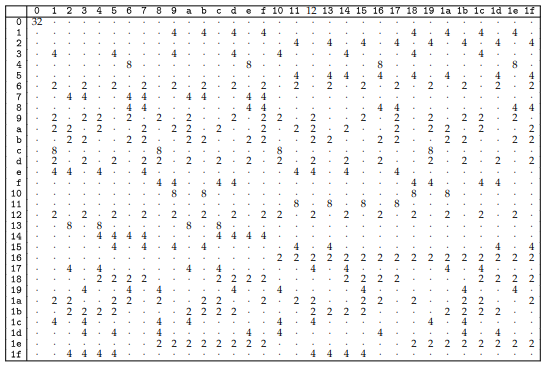
\includegraphics[width=12cm]{images/ddt.png}
    \caption[short]{DDT}
\end{figure}
\begin{figure}[h!]
    \centering
    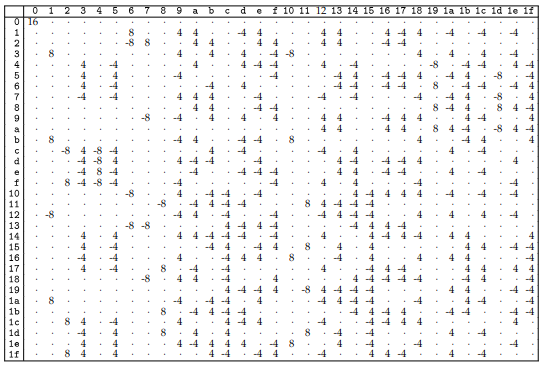
\includegraphics[width=12cm]{images/lat.png}
    \caption[short]{LAT}
\end{figure}

\newpage